\begin{frame}{overflow and undefined behavior}
\begin{itemize}
\item C standard: some things are \textit{undefined behavior}
\item C compiler can do anything in those cases
\vspace{.5cm}
\item \textit{signed integer overflow} is undefined
\item \textit{unsigned integer overflow} must wrap around
\end{itemize}
\end{frame}

\begin{frame}[fragile]{-fsanitize=undefined}
\begin{Verbatim}[fontsize=\small]
int x = INT_MAX -1; int y = 5; printf("%d\n", x * y);
\end{Verbatim}
\begin{itemize}
\item compile with \texttt{-fsanitize=undefined}:
    \begin{itemize}
        \item \texttt{test.c:...: runtime error: signed integer overflow: 2147483646 * 5 cannot be represented in type 'int}
    \end{itemize}
\item compile with \texttt{-ftrapv}: \texttt{Aborted (core dumped)}
\end{itemize}
\begin{Verbatim}[fontsize=\small]
unsigned x = INT_MAX -1; unsigned y = 5; printf("%u\n", x * y);
\end{Verbatim}
\begin{itemize}
\item compile with \texttt{-fsanitize=undefined} or \texttt{-ftrapv}: NO ERROR
\end{itemize}
\end{frame}

\begin{frame}[fragile]{in Rust (1)}
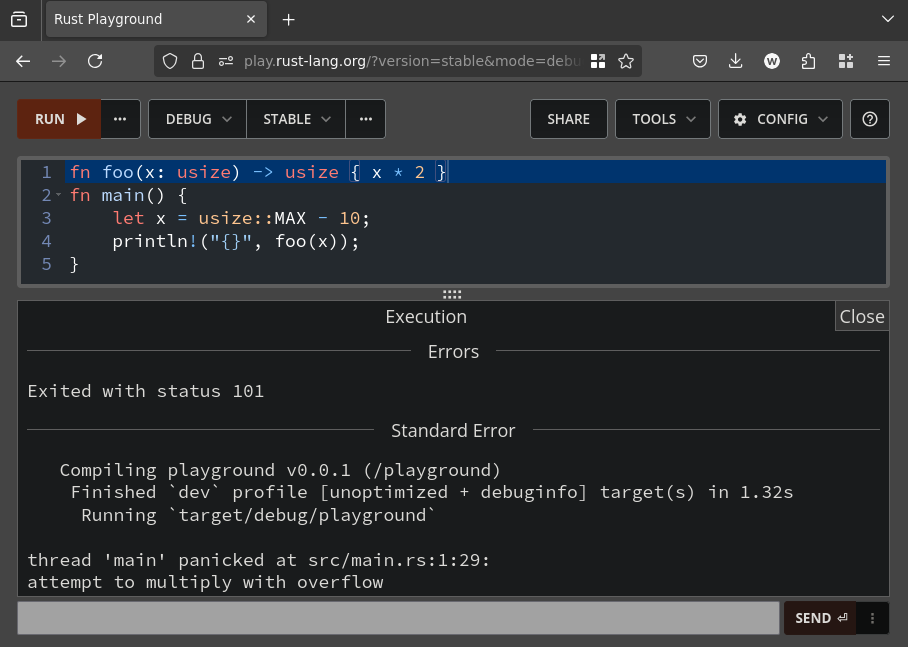
\includegraphics[height=0.9\textheight]{../overflow-int/rust-oflow-trap}
\end{frame}

\begin{frame}[fragile]{in Rust (2)}
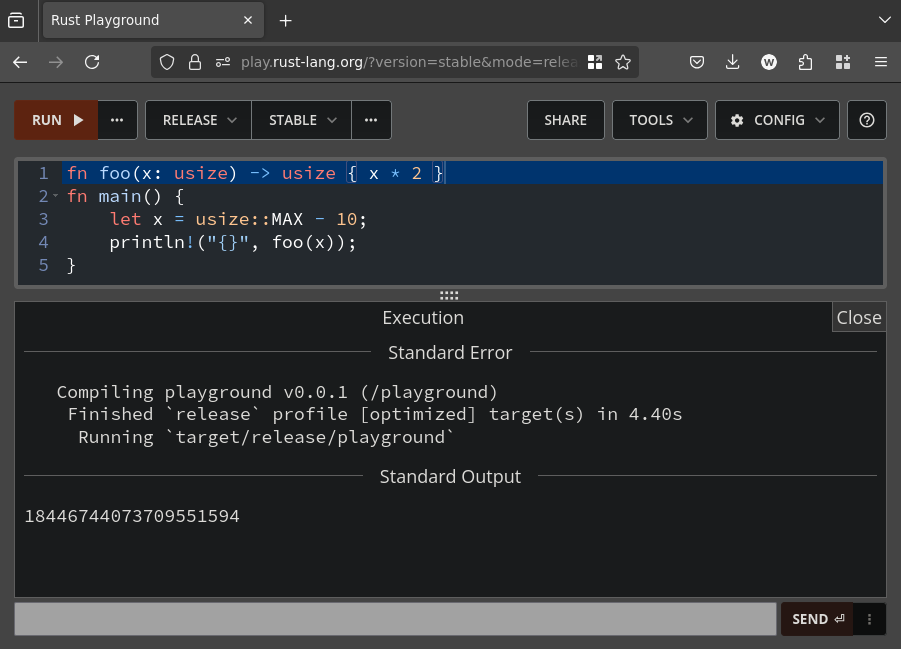
\includegraphics[height=0.9\textheight]{../overflow-int/rust-oflow-notrap}
\end{frame}

\begin{frame}[fragile]{in Rust (3)}
\begin{Verbatim}[fontsize=\fontsize{11}{12}]
let x = usize::MAX - 10; let y = 10usize;
println!("{} {}", x.saturating_mul(2), y.saturating_mul(2));
// 18446744073709551615 20
    // 18446744073709551615==usize::MAX
println!("{:?} {:?}", x.checked_mul(2), y.checked_mul(2));
// None Some(30)
println!("{} {}", x.wrapping_mul(2), y.wrapping_mul(2));
// 18446744073709551594 20
    // 18446744073709551594==usize::MAX-21
\end{Verbatim}
\end{frame}
